\chapter{Results}
\label{results}

\section{Phase One Results}
\label{results:userStudyPhaseOne}

In this phase, we recorded \uniqueUsersPhaseOneUserStudy users reciting any of the \numOronymsPhaseOneUserStudy  oronyms of the phrase ``an ice cold hour'', or any of the \numForthRightOohOronymPhrases oronyms for the phrase ``fourth rye to''.  Out of \numResponsesPhaseOneUserStudy recordings, only the recordings of the oronyms of ``fourth rye to" were found to diverge from our excepted phonetic patterns, likely due to poor microphone quality not being able to pick up the aspriated \emph{`f'} sound at the beginning of the phrase\cite{elko_electronic_2007}. All other oronyms were found to be within reasonable tolerance levels, with \recordingsPhaseTwoUserStudy recordings from one particular speaker found to be a close enough match to the general American accent to use his recordings in phase two.


\section{Phase Two Results}
\label{results:userStudyPhaseTwo}


We gathered \numTotalTranscriptionsPhaseTwo transcriptions for our \recordingsPhaseTwoUserStudy recorded phrases, with each recording garnering \numTranscriptionsPerRecordingPhaseTwoUserStudy transcriptions each.  Worldwide, the top four most-frequently transcribed phrases made up for 70\% of total transcriptions.  The top transcribed phrase worldwide was ``an ice cold hour'', with \phaseTwoUserStudyTimesTranscribedAnIceColdHour transcriptions, followed by  ``a nice cold hour'', with \phaseTwoUserStudyTimesTranscribedANiceColdHour transcriptions.  Following that, ``a nice gold hour'' had \phaseTwoUserStudyTimesTranscribedANiceGoldHour transcriptions, and ``in ice cold hour'' had \phaseTwoUserStudyTimesTranscribedInIceColdHour transcriptions. The breakdown of these top four can be seen in figure ~\ref{fig:mostCommonTranscriptionsPieChartGlobal} and table ~\ref{table:fullFreqVsActual}. 

All of the worldwide top transcribed phrases were predicted by our oronym-generator, except for ``a nice gold hour''.  This is a known limitation of our project, though, because we chose to focus on exact phonetic matches.  The cold/gold mishearing is a product of phoneme voiced/voiceless pair swapping, which we cover in-depth in section ~\ref{section:phonemeSwapping}. It is outside the current scope of our project. 


\begin{figure}
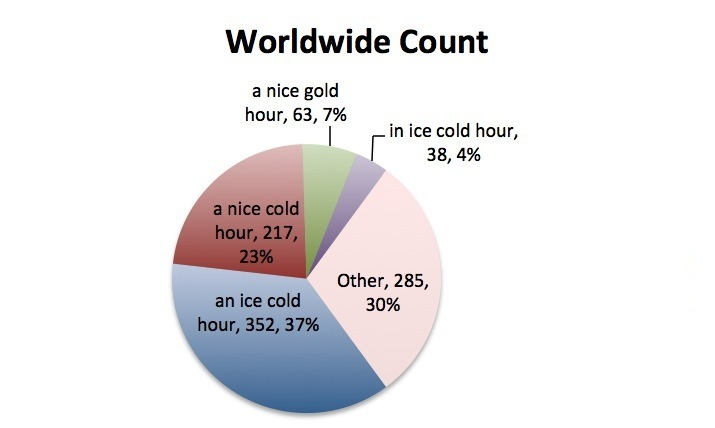
\includegraphics[width=150mm]{PieChart_WorldwideCount_noBar.jpg}
\captionfonts
\caption[Most Common Transcriptions Globally]{ Our top two transcriptions were ``a nice cold hour'' and ``an ice cold hour'' }
\label{fig:mostCommonTranscriptionsPieChartGlobal}
\end{figure}


\begin{table}
\begin{center}
\begin{tabular}{ | l | l | l | c | }
\hline 
predicted freq & phrase transcribed & total answers \\
\hline 
931028 &  an ice cold hour &  \phaseTwoUserStudyTimesTranscribedAnIceColdHour \\
\hline
7851662&   a nice cold hour &  \phaseTwoUserStudyTimesTranscribedANiceColdHour  \\
\hline
0  & a nice gold hour &  \phaseTwoUserStudyTimesTranscribedANiceGoldHour \\
\hline
5503158&   in ice cold hour &  \phaseTwoUserStudyTimesTranscribedInIceColdHour \\
\hline
0 &  an ice gold hour &  \phaseTwoUserStudyTimesTranscribedAnIceGoldHour \\
\hline
859307 &  an eye scold hour &  \phaseTwoUserStudyTimesTranscribedAnEyeScoldHour \\
\hline 
\end{tabular}
\captionfonts
\caption[Phrase word frequency sum vs times transcribed]{ In this table, we list all oronyms that were transcribed more than five times. Out of this list, all but the two containing the word ``gold" were predicted by our oronym algorithm.  However, we expected that any voiced/voiceless phoneme substitutions, like ``cold''/``gold'' would be missed by our algorithm. }
\label{table:fullFreqVsActual}
\end{center}
\end{table}


%\begin{figure}
%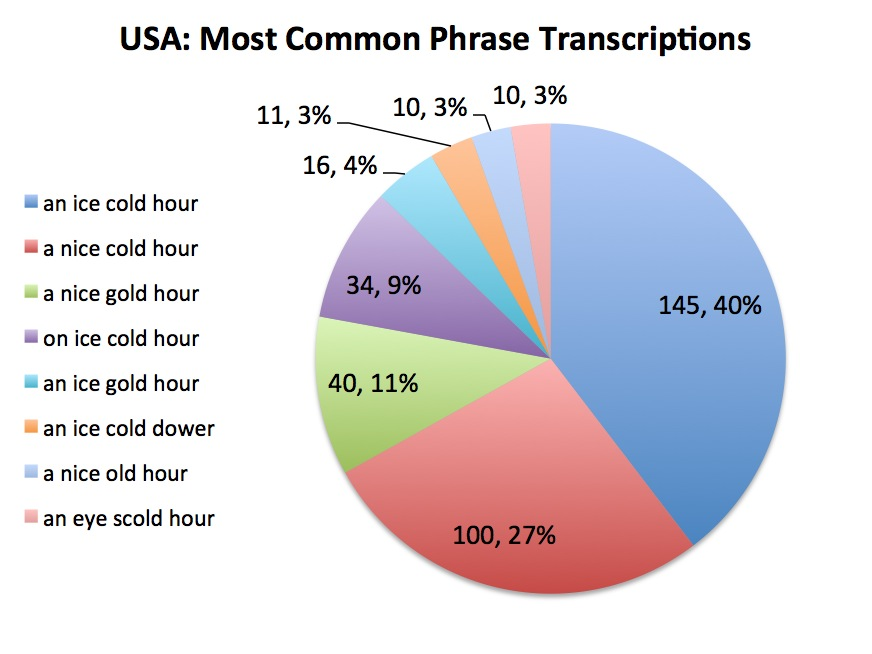
\includegraphics[width=150mm]{mostCommonTranscriptionsPieChartUSA.jpg}
%\captionfonts
%\caption[Most Common Transcriptions from American respondents]{ Though the breakdown is a bit different than the global transcription breakdown, you can still see the clear trend of ``a nice cold hour" and ``an ice cold hour" being the most common.  There is a slightly larger gap between these two phrase, we hypothesize, because the American transcribers are familiar with what words normally are in proximity to others. }
%\label{fig:mostCommonTranscriptionsPieChartUSA}
%\end{figure}



\subsection{Transcribed oronyms' observed frequency vs expected frequency}
\label{results:transcriptionExpectedVsObservedFreq}

Though the most commonly transcribed phrases were predicted by our method of oronym generation, figure ~\ref{fig:results:aNiceColdHourObserved} shows an unexpected distribution of the number of times each phrase was transcribed versus the frequency metric that we calculated. We hypothesized that a simple summation of the UNISYN-provided word frequencies for each word in a phrase would produce a meaningful indicator of whether a phrase's likelyhood to be heard.  

\begin{figure}
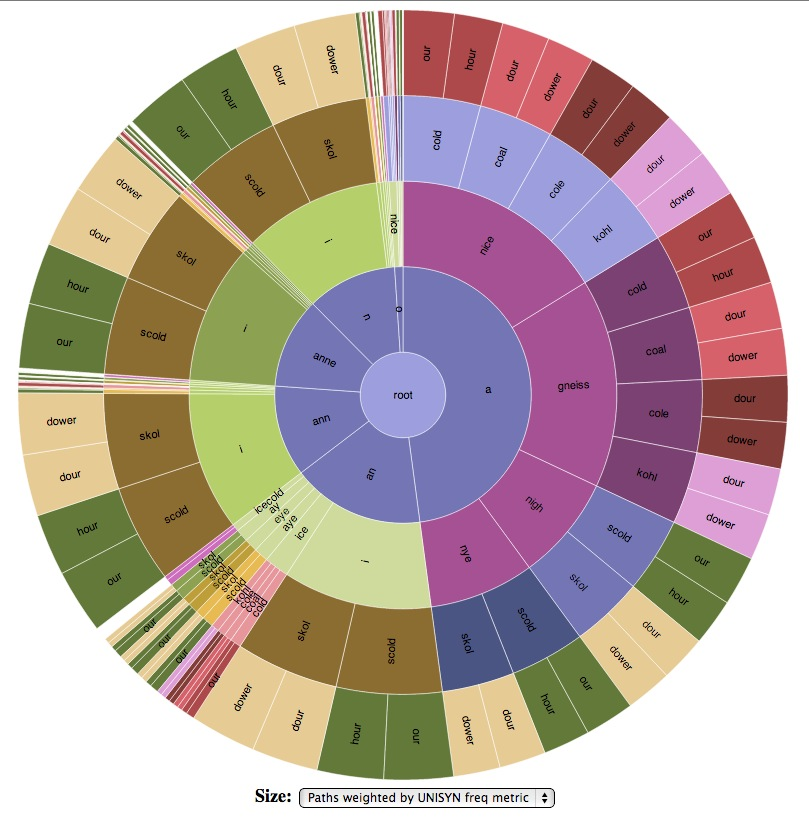
\includegraphics[width=150mm]{aNiceColdHour_UNISYN_FreqMetric_withUnpredictedSliver.jpg}
\captionfonts
\caption[Sunburst Chart for A Nice Cold Hour using UNISYN metrics for comparison to observed frequency sunburst]{Sunburst Chart for A Nice Cold Hour using UNISYN metrics for comparison to observed frequency sunburst}
\label{fig:results:aNiceColdHourUNISYNwithUnpredicted}
\end{figure}

\begin{figure}
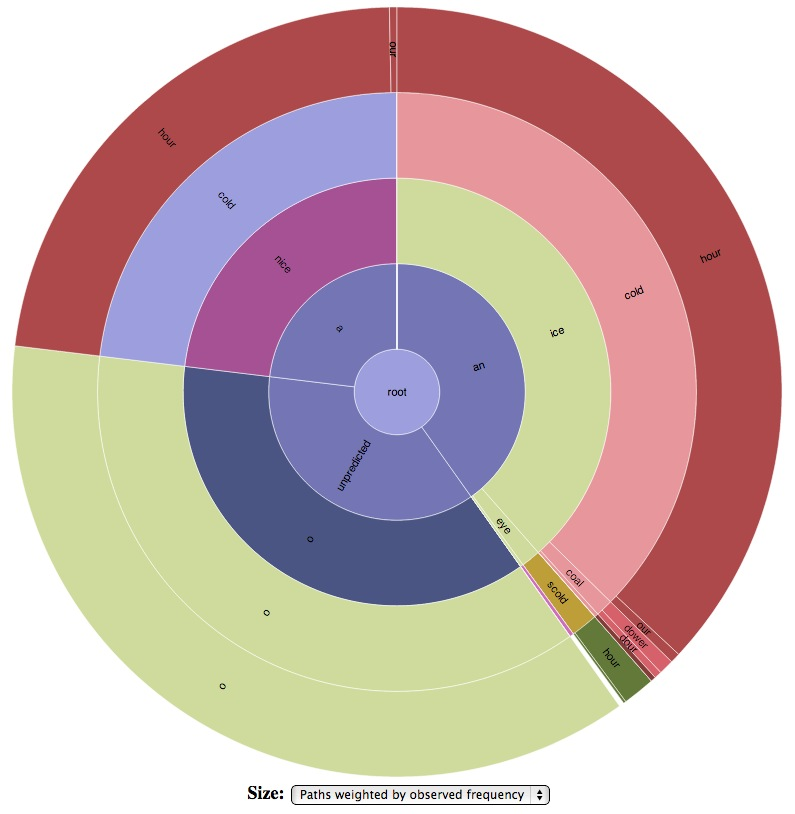
\includegraphics[width=150mm]{aNiceColdHour_Observed.jpg}
\captionfonts
\caption[Sunburst Chart for A Nice Cold Hour using observed frequencies]{Sunburst Chart for A Nice Cold Hour using observed frequencies}
\label{fig:results:aNiceColdHourObserved}
\end{figure}


Unfortunately, that proved not to be the case.  In figure ~\ref{fig:results:aNiceColdHourUNISYNwithUnpredicted}, we see the sunburst diagram for the expected distribution of transcribed phrases based upon the UNISYN frequency metric that we calculated.  In figure ~\ref{fig:results:aNiceColdHourObserved}, we see the sunburst diagram for the transcriptions we observed, with a special slice representing all the transcriptions we did not predict. The unpredicted slice is nearly as large as the slice for ``an ice cold hour'', which was observed the most often out of all expected transcriptions. 


\subsection{Statistical measurement of expected versus observed transcription frequency}
\label{results:statisticsINYOURFACE}


A statistical analysis of the observed dataset versus the expected dataset, using a one-proportion z test, further proves that the calculated UNISYN frequency values were not a good predictor of observed transcription.   Using the top two observed transcriptions as our sample population, we take a look at the phrases \phraseOne and \phraseTwo.  The phrase \phraseOne has a calculated UNISYN freq metric of \unisynFreqForPhraseOne, and had \USATranscriptionsOfPhraseOne actual transcriptions observed among people living in the United States. The phrase \phraseTwo has a calculated UNISYN freq metric of \unisynFreqForPhraseTwo, and had \USATranscriptionsOfPhraseTwo actual transcriptions observed among people living in the United States. Therefore, the expected population is \unisynCombinedFreq, and the observed population is \USACombinedTranscriptions.  

Given those population, the expected population proportion for \phraseOne would be \unisynFreqForPhraseOne  $\div$ \unisynCombinedFreq, or \expectedProportionOfPhraseOneOccurances.  

In our user study, we found that \USATranscriptionsOfPhraseOne people transcribed \phraseOne, and \USATranscriptionsOfPhraseTwo people transcribed \phraseTwo, for a ratio of 0.65 to 1, where \phraseOne accounts for 39.56\% ( p = \observedProportionOfPhraseOneOccurances ) of the combined count. 

Given the observed population proportion of \observedProportionOfPhraseOneOccurances and the expected population proportion \expectedProportionOfPhraseOneOccurances, we did a one-proportion z test with an $\alpha$ of \alphaSigFigs.  The z value returned was \UNISYNzVal, meaning that the observed population proportion was \UNISYNzVal standard deviations away from the expected population proportion.  When we used this z value to compute a p value, we got a value so low that we were unable find a calculator with enough decimal places to show it without rounding it to zero.

In short, the per-occurance frequency metric predictions derived from UNISYN don't even remotely match the observed data.


The below is here mostly for my edification: (I'll delete it when my edits are all done.)

Givens for Phrase (1) (\phraseOne) :

Calculated metric: \unisynFreqForPhraseOne

Actual count: x = \USATranscriptionsOfPhraseOne


Givens for Phrase (2) (\phraseTwo) :

Calculated metric: \unisynFreqForPhraseTwo

Actual count: x = \USATranscriptionsOfPhraseTwo

$\alpha$ = significance Level = \alphaSigFigs

Calculated sum: \unisynFreqForPhraseOne + \unisynFreqForPhraseTwo =  \unisynCombinedFreq

Actual sum: \USATranscriptionsOfPhraseOne + \USATranscriptionsOfPhraseTwo = \USACombinedTranscriptions

p = population proportion of \phraseOne occurrences

p = \unisynFreqForPhraseOne   $\div$  \unisynCombinedFreq  = \pvalue 

$H_{o}$ :  p = \pvalue 
$H_{a}$ :  p $\neq$ \pvalue 

Actual: 
\USATranscriptionsOfPhraseOne  $\div$ \USACombinedTranscriptions  = 

1-proportion z-test

z = \UNISYNzVal std deviations away from expected.

If pvalue < $\alpha$, reject $H_{o}$

pvalue $\approx$ 0 < \alphaSigFigs

So, reject $H_{o}$


\subsection{Observations on Transcription Count per Recording for each transcribed phrase}
\label{results:transcriptionCountPerRecording}

The Transcription Count by Recording graphs show how many occurances of a certain transcription were produced from each recording. Each graph represents one transcription, and has bars for each recording, where each bar shows how many times the transcription was observed for that particular recording. The graph also compares the observed incidences of those transcriptions with the expected UNISYN frequency metric. The X axis lists the transcribed phrase.  The right Y axis corresponds to the smaller, multi-colored bars. Each bar represents the number of times that a transcribed phrase was observed for that particular recording. 
The left X axis corresponds to the large blue bar behind the smaller bars. The blue bar represents the calculated UNISYN frequency metric for the transcription.


When you compare the bars from the two y axes, some interesting patterns appear. 

\subsubsection{An ice cold hour}
\label{results:transcriptionCountPerRecording:an_ice_cold_hour}

When looking at figure ~\ref{fig:results:transcriptionCountPerRecordingAnIceColdHour}, we notice that all but 12 out of the 362 transcriptions of ``an ice cold hour'' come from recordings of phrases that similarly begin with ``an''. This suggests the existence of some un-measured value related to pronunciation that makes the theoretically identical phonetic sequences of ``an ice cold hour'' and ``a nice cold hour'' be heard as functionally different. Also, note that in figure ~\ref{fig:results:transcriptionCountPerRecordingAnIceColdHour}, the blue bar representing the UNISYN frequency prediction for the transcribed phrase underpredicts the number of transcriptions from recordings that begin with ``an'', while doing a fairly good job of predicting transcription incidence for recordings that begin with ``a''.


\begin{figure}
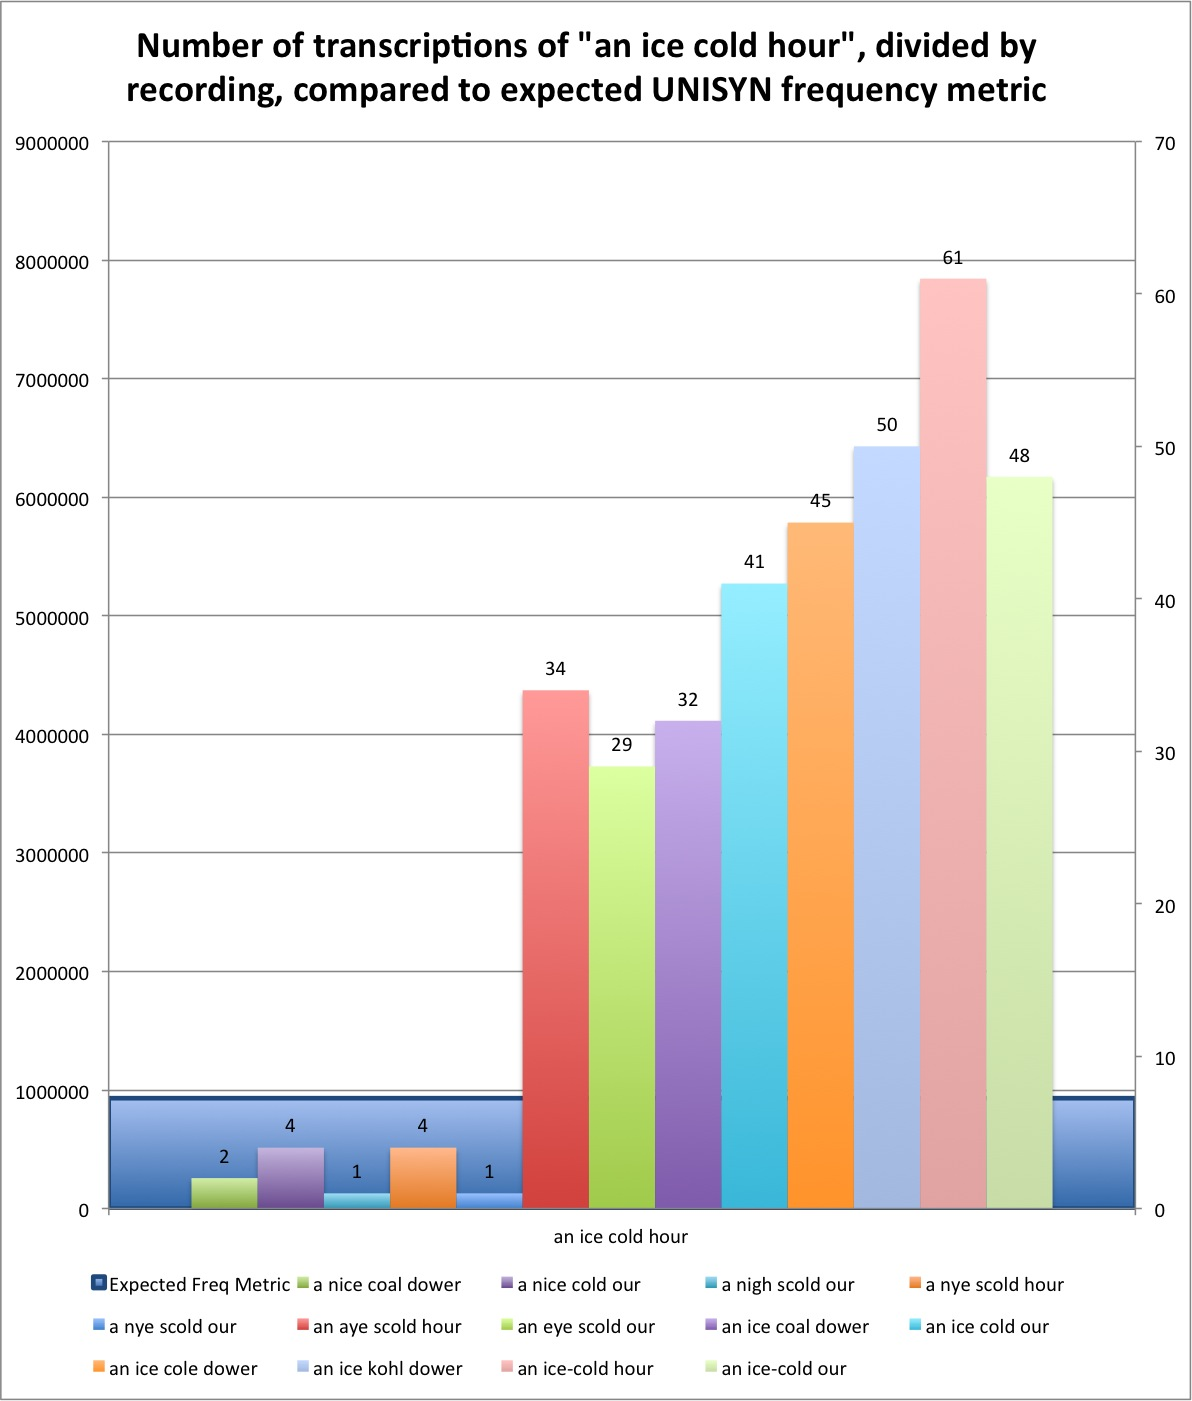
\includegraphics[width=\textwidth]{TranscriptionCountPerRecording_an_IceColdHour.jpg}
\captionfonts
\caption[Transcription Count Per Recording for the transcribed phrase ``an ice cold hour'']{ This graph represents all transcriptions of the phrase ``an ice cold hour'', divided into columns based on what recording were transcribed as ``an ice cold hour''. The large blue bar in the background shows the predicted frequency metric for the phrase in question.}
\label{fig:results:transcriptionCountPerRecordingAnIceColdHour}
\end{figure}

\subsubsection{A nice cold hour}
\label{results:transcriptionCountPerRecording:a_nice_cold_hour}

In figure ~\ref{fig:results:transcriptionCountPerRecordingANiceColdHour}, we see that, while most of the transcriptions of ``a nice cold hour'' came from recordings of phrases that begin with 'a', a not-inconsiderable number came from the recordings for the phrases ``an ice cold our'' and ``an ice-cold our''. When taken in regards to the conclusions we drew from figure ~\ref{fig:results:transcriptionCountPerRecordingAnIceColdHour} in section ~\ref{results:transcriptionCountPerRecording:an_ice_cold_hour}, we can conclude that, while listeners appear not to be able to hear an `a' as an `an', listeners can, under certain circumstances, hear an `an' as an `a'.  The blue prediction bar shows that the expected incidence over all recordings was much higher than the observed incidence, and only came close to being correct for the recorded phrases ``a nice cold hour'' and ``a nice coal dower''.

\begin{figure}
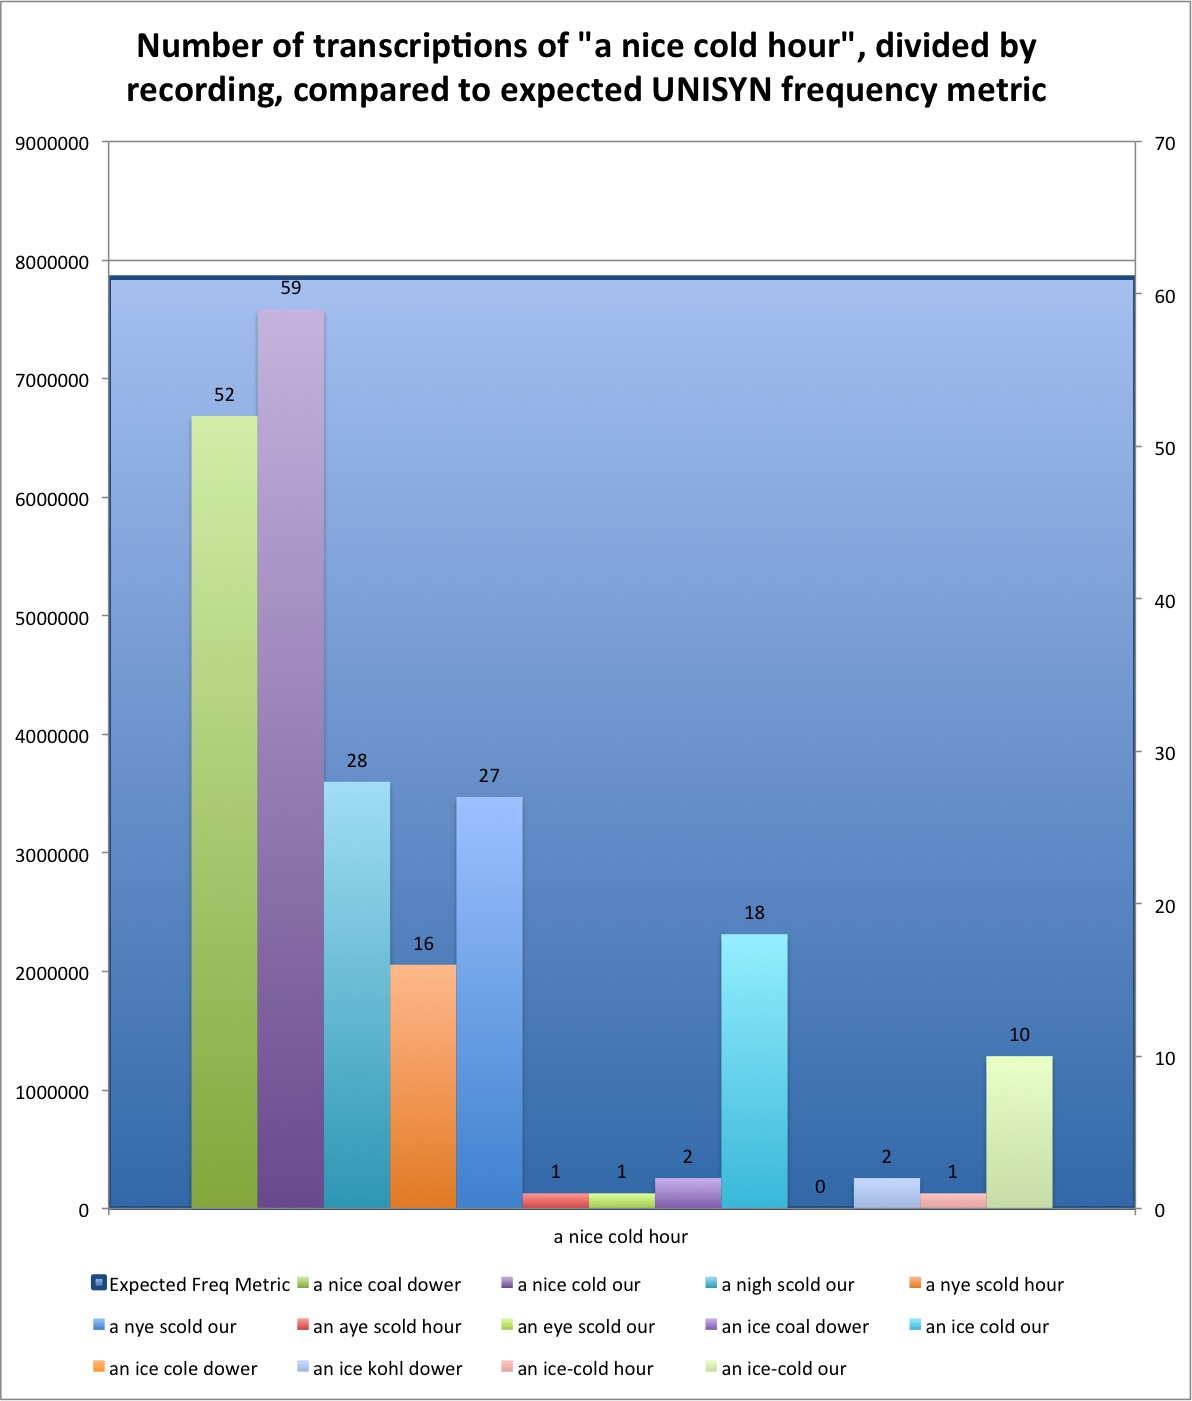
\includegraphics[width=\textwidth]{TranscriptionCountPerRecording_a_NiceColdHour.jpg}
\captionfonts
\caption[Transcription Count Per Recording for the transcribed phrase ``a nice cold hour'']{ This graph represents all transcriptions of the phrase ``a nice cold hour'', divided into columns based on what recording were transcribed as ``a nice cold hour''. The large blue bar in the background shows the predicted frequency metric for the phrase in question.}
\label{fig:results:transcriptionCountPerRecordingANiceColdHour}
\end{figure}



\subsubsection{In ice cold hour}
\label{results:transcriptionCountPerRecording:in_ice_cold_hour}

This chart in figure ~\ref{fig:results:transcriptionCountPerRecordingInIceColdHour} is for the third most common transcription, ``in ice cold hour''.  Transcriptions of this phrase are fairly evenly distributed among the recordings, though there is a spike of transcriptions on  ``an ice-cold hour''.  Additionally, similar to earlier observations, the transcriptions occur a lot less frequently than the UNISYN frequency metric bar suggests they should.

\begin{figure}
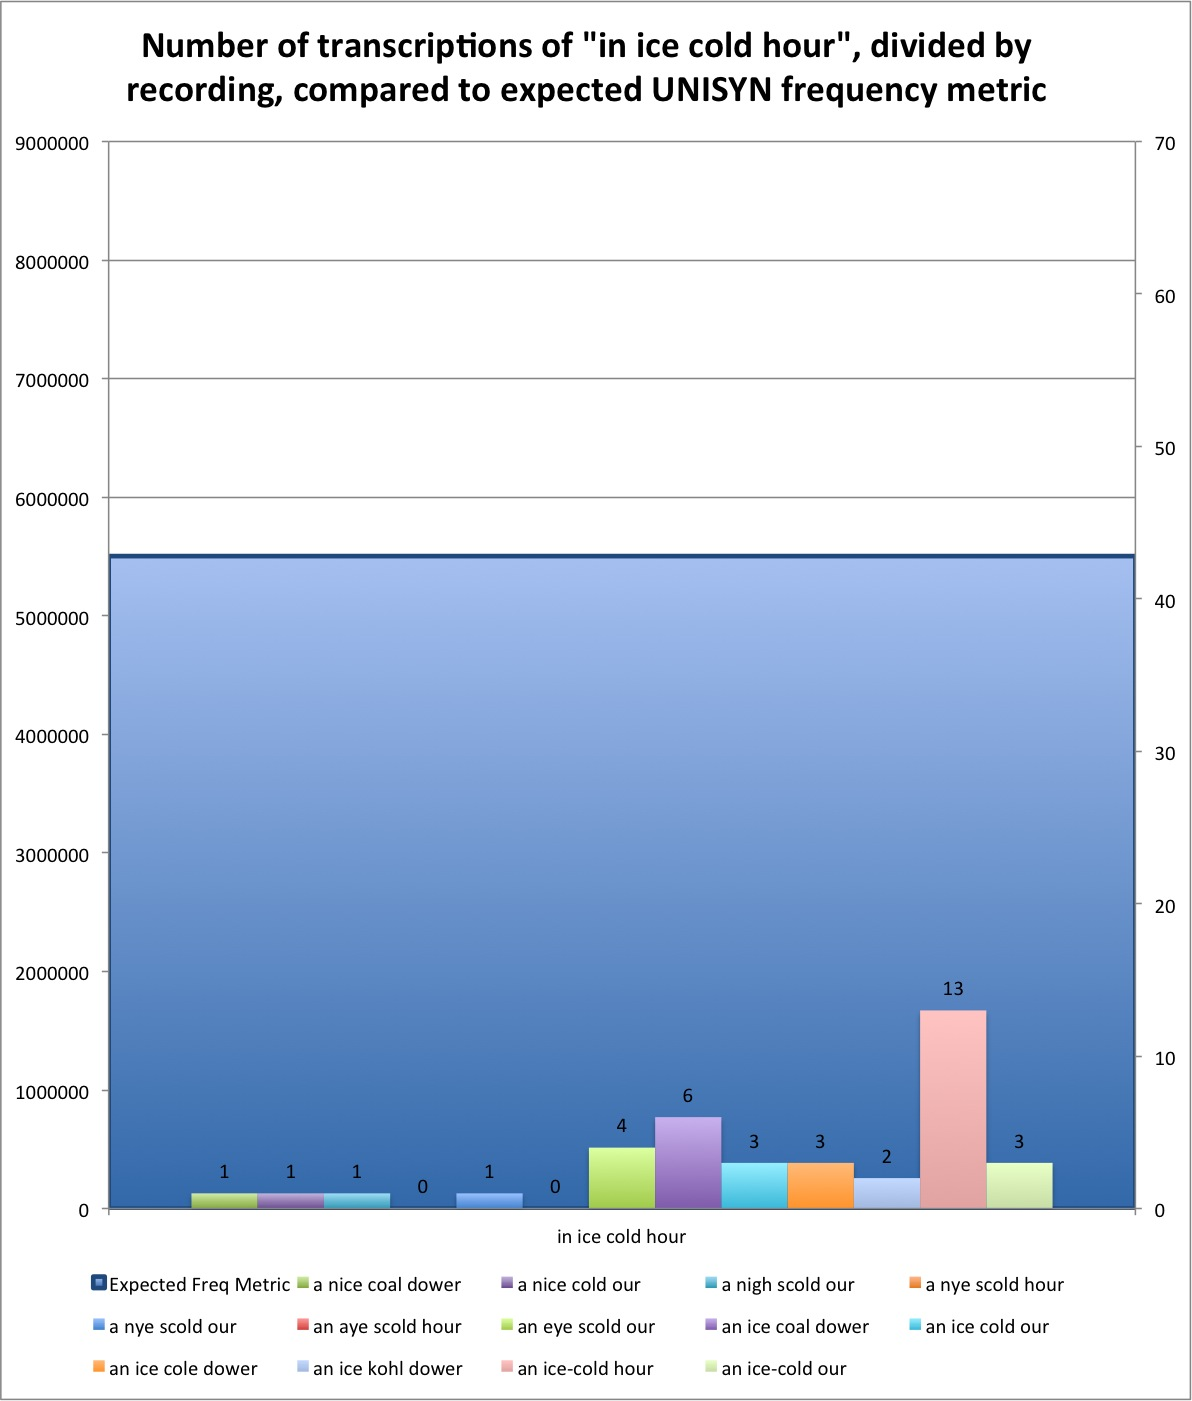
\includegraphics[width=\textwidth]{TranscriptionCountPerRecording_inIceColdHour.jpg}
\captionfonts
\caption[Transcription Count Per Recording for the transcribed phrase ``in ice cold hour'']{ This graph represents all transcriptions of the phrase ``in ice cold hour'', divided into columns based on what recording were transcribed as ``in ice cold hour''. The large blue bar in the background shows the predicted frequency metric for the phrase in question.}
\label{fig:results:transcriptionCountPerRecordingInIceColdHour}
\end{figure}



\subsubsection{A nice gold hour}
\label{results:transcriptionCountPerRecording:a_nice_gold_hour}

The chart in figure ~\ref{fig:results:transcriptionCountPerRecordingANiceGoldHour} for the transcriptions of ``a nice gold hour'' shows that the source recordings of those transcriptions are very specific: only the recordings of ``a nye scold our'', ``a nye scold hour'', and ``a nigh scold our'' produce the 'g'/'c' substitution. In fact, all of our transcriptions that involved the word ``gold'' arose from these recordings. This suggests a relationship between the phonemes \texttt{s k} and \texttt{g}, and warrants further investigation, as suggested later in section ~\ref{section:phonemeSwapping}. As shown by the lack of a background blue bar in this diagram, this transcription was not predicted by our oronym generation algorithm, due to the aforementioned phoneme swapping.

\begin{figure}
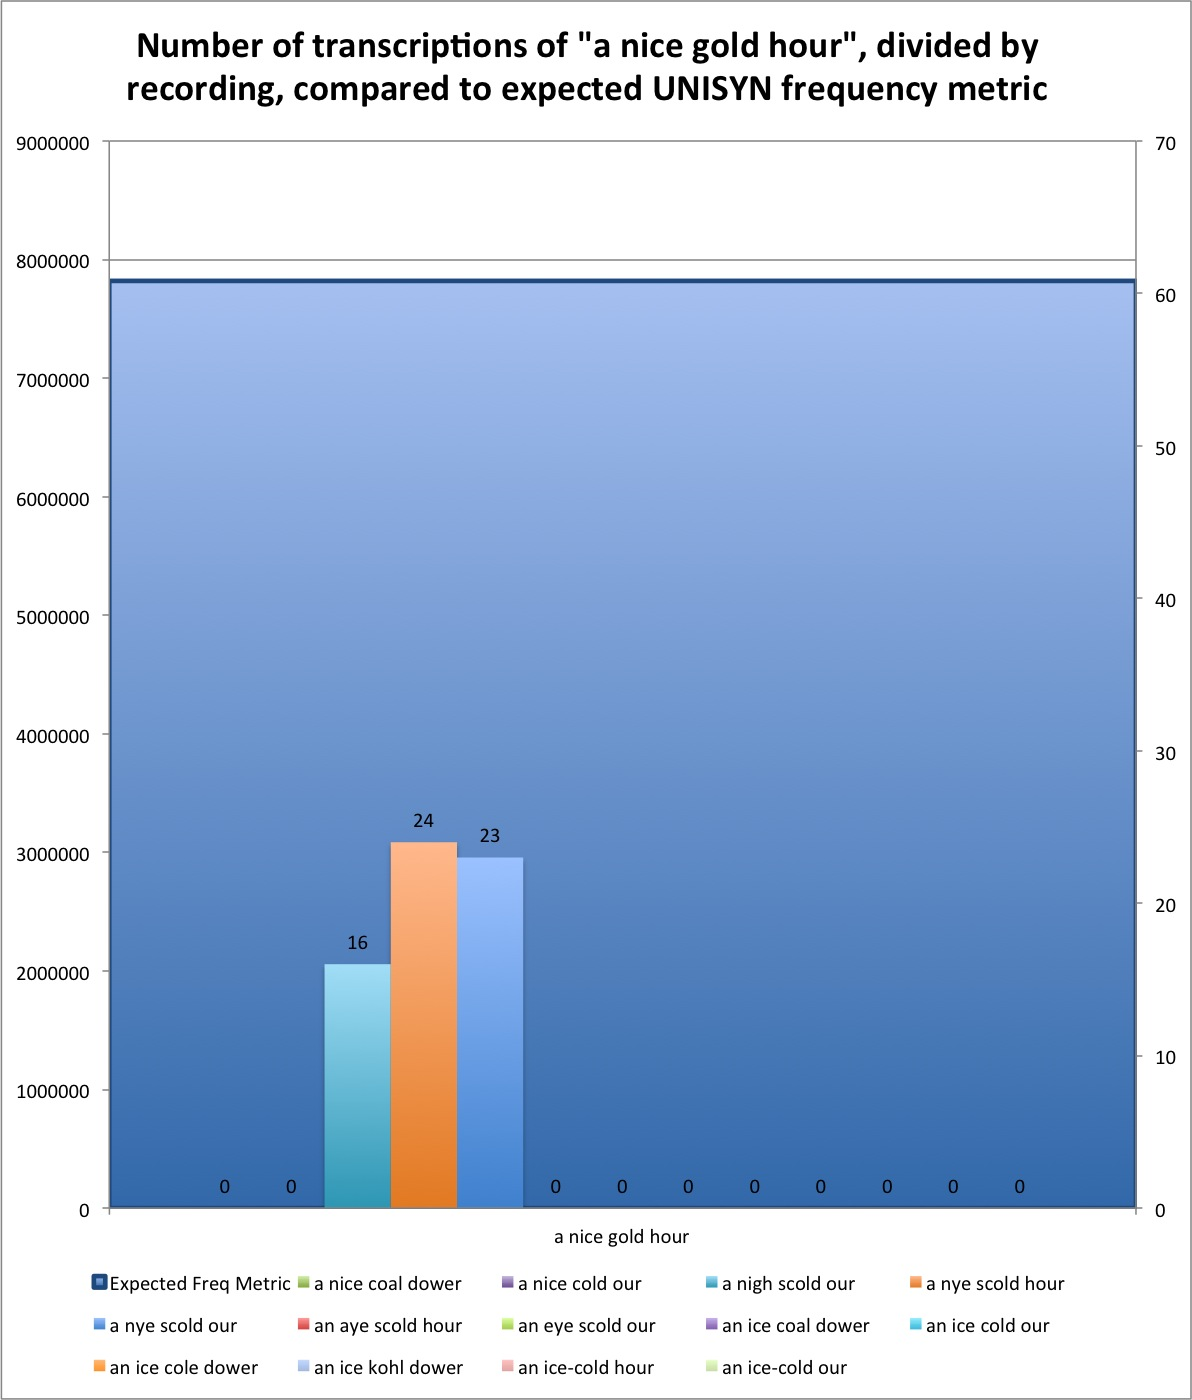
\includegraphics[width=\textwidth]{TranscriptionCountPerRecording_aNiceGoldHour.jpg}
\captionfonts
\caption[Transcription Count Per Recording for the transcribed phrase ``a nice gold hour'']{ This graph represents all transcriptions of the phrase ``a nice gold hour'', divided into columns based on what recording were transcribed as ``a nice gold hour''. The large blue bar in the background shows the predicted frequency metric for the phrase in question.}
\label{fig:results:transcriptionCountPerRecordingANiceGoldHour}
\end{figure}


\subsubsection{An ice cold dower}
\label{results:transcriptionCountPerRecording:an_ice_cold_dower}

Figure ~\ref{fig:results:transcriptionCountPerRecordingANiceColdDower} shows the transcriptions for the phrase ``an ice cold dower''. This phrase features repeated-phoneme auto-deletion or auto-insertion. Repeated-phoneme auto-deletion or -insertion occurs when two identical and adjacent phonemes are blurred into one sound.  This can result in the listener putting two phonemes where only one exists (as in this case), or putting one phoneme where two exist. This phenomenon, while known to us, is outside the scope of the current project, and suggested for future work.  Due to this limit in scope, this transcription was not predicted by our oronym generation algorithm, as shown by the lack of a background blue frequency prediction bar in figure ~\ref{fig:results:transcriptionCountPerRecordingANiceColdDower}.

\begin{figure}
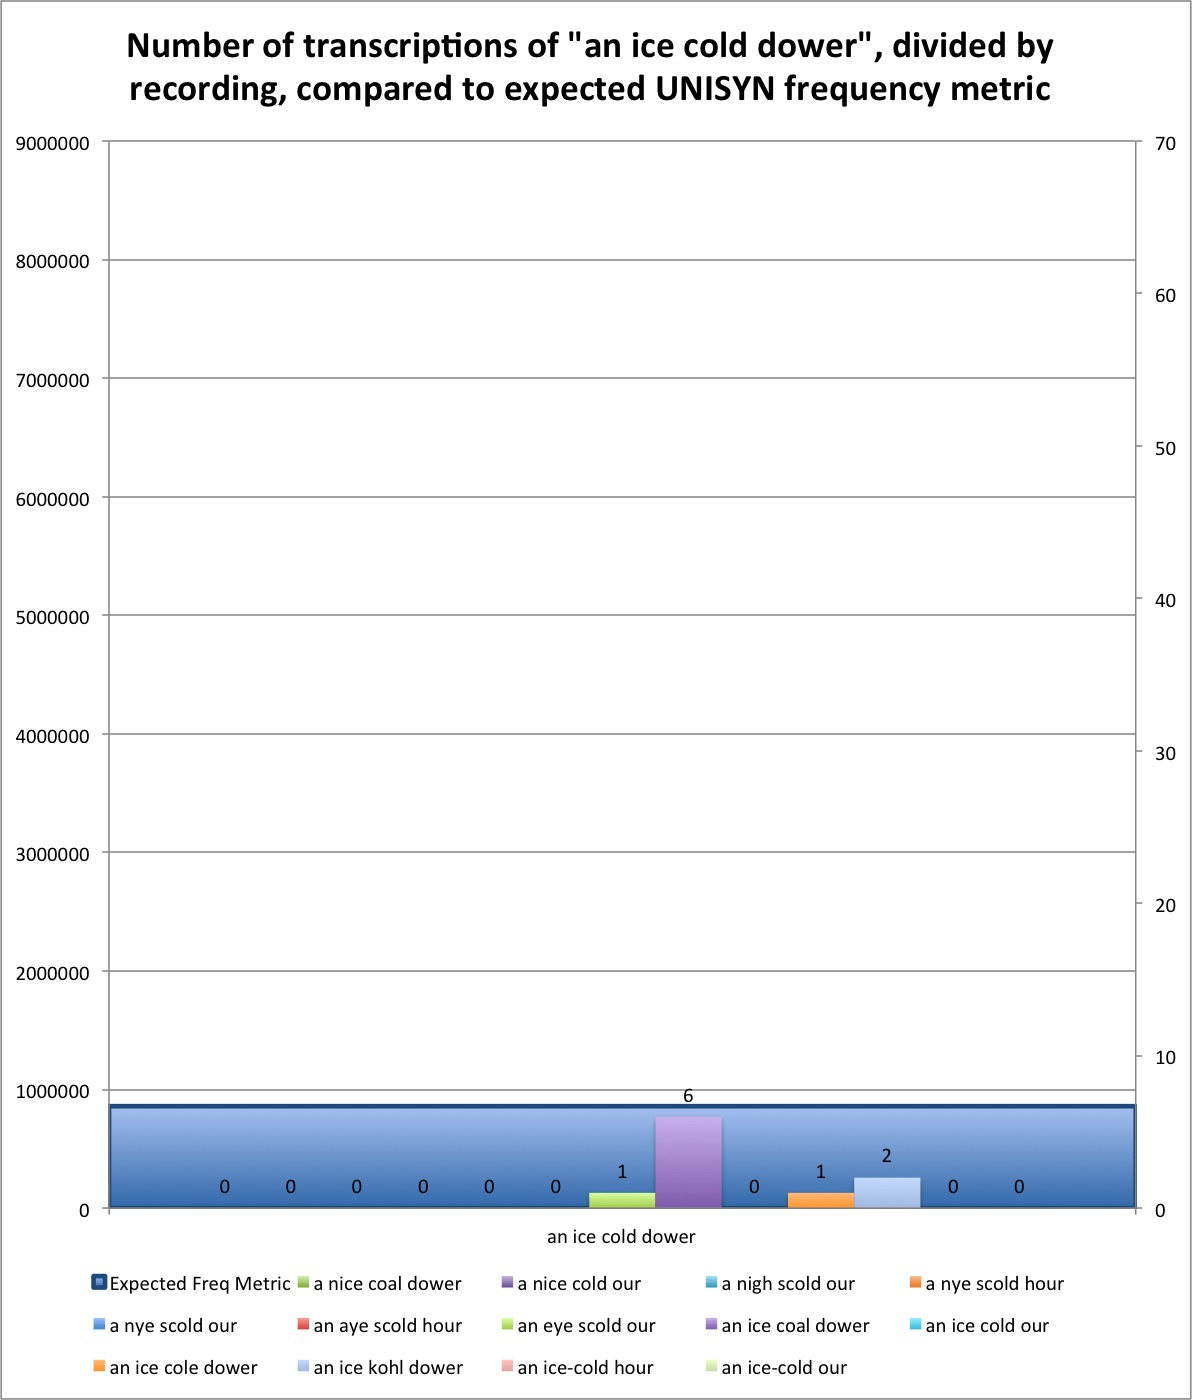
\includegraphics[width=\textwidth]{TranscriptionCountPerRecording_anIceColdDower.jpg}
\captionfonts
\caption[Transcription Count Per Recording for the transcribed phrase ``a nice cold dower'']{ This graph represents all transcriptions of the phrase ``a nice cold dower'', divided into columns based on what recording were transcribed as ``a nice cold dower''. The large blue bar in the background shows the predicted frequency metric for the phrase in question.}
\label{fig:results:transcriptionCountPerRecordingANiceColdDower}
\end{figure}


\subsubsection{An eye scold hour}
\label{results:transcriptionCountPerRecording:an_eye_scold_hour}

The chart for ``an eye scold hour'', shown in figure ~\ref{fig:results:transcriptionCountPerRecordingAnEyeScoldHour}, is primarily interesting in that it appears more or less deterministically interpretable. The only recordings that resulted in this phrase were those for ``an eye scold hour'' or ``an aye scold hour''. We hypothesize that this has something to do with word emphases, and suggest investigating this for future work. Interestingly enough, the predicted frequency value (scaled) was fairly close to the actual occurance for that phrase.


\begin{figure}
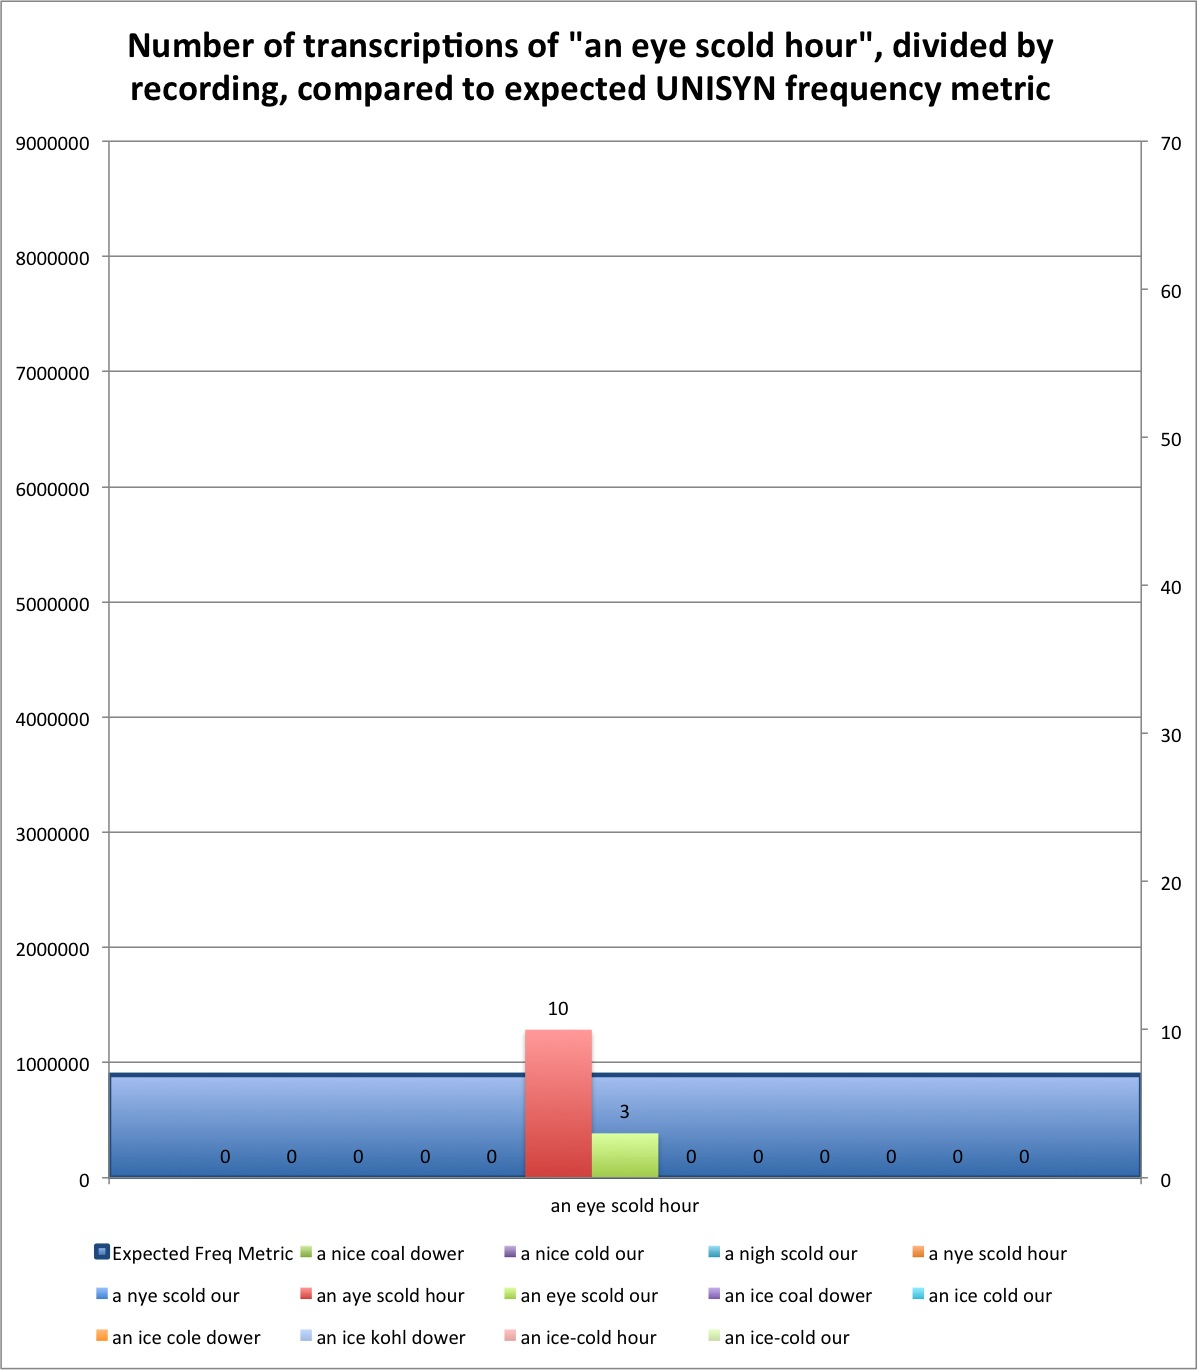
\includegraphics[width=\textwidth]{TranscriptionCountPerRecording_anEyeScoldHour.jpg}
\captionfonts
\caption[Transcription Count Per Recording for the transcribed phrase ``an eye scold hour'']{ This graph represents all transcriptions of the phrase ``an eye scold hour'', divided into columns based on what recording were transcribed as ``an eye scold hour''. The large blue bar in the background shows the predicted frequency metric for the phrase in question.}
\label{fig:results:transcriptionCountPerRecordingAnEyeScoldHour}
\end{figure}

\subsubsection{An ice coal dower}
\label{results:transcriptionCountPerRecording:an_ice_coal_dower}

The chart for ``an ice coal dower'' in figure ~\ref{fig:results:transcriptionCountPerRecordingAnIceCoalDower} is notable in that all its transcriptions came from recordings that began in ``an'' and ended in ``dower'', like the phrase itself does. As in ~\ref{fig:results:transcriptionCountPerRecordingAnEyeScoldHour}, we suggest that the near-deterministic interpretation has something to do with emphases, and suggest investigating this for future work. The UNISYN frequency metric once again predicted higher expected incidences than were actually observed for this transcription.

\begin{figure}
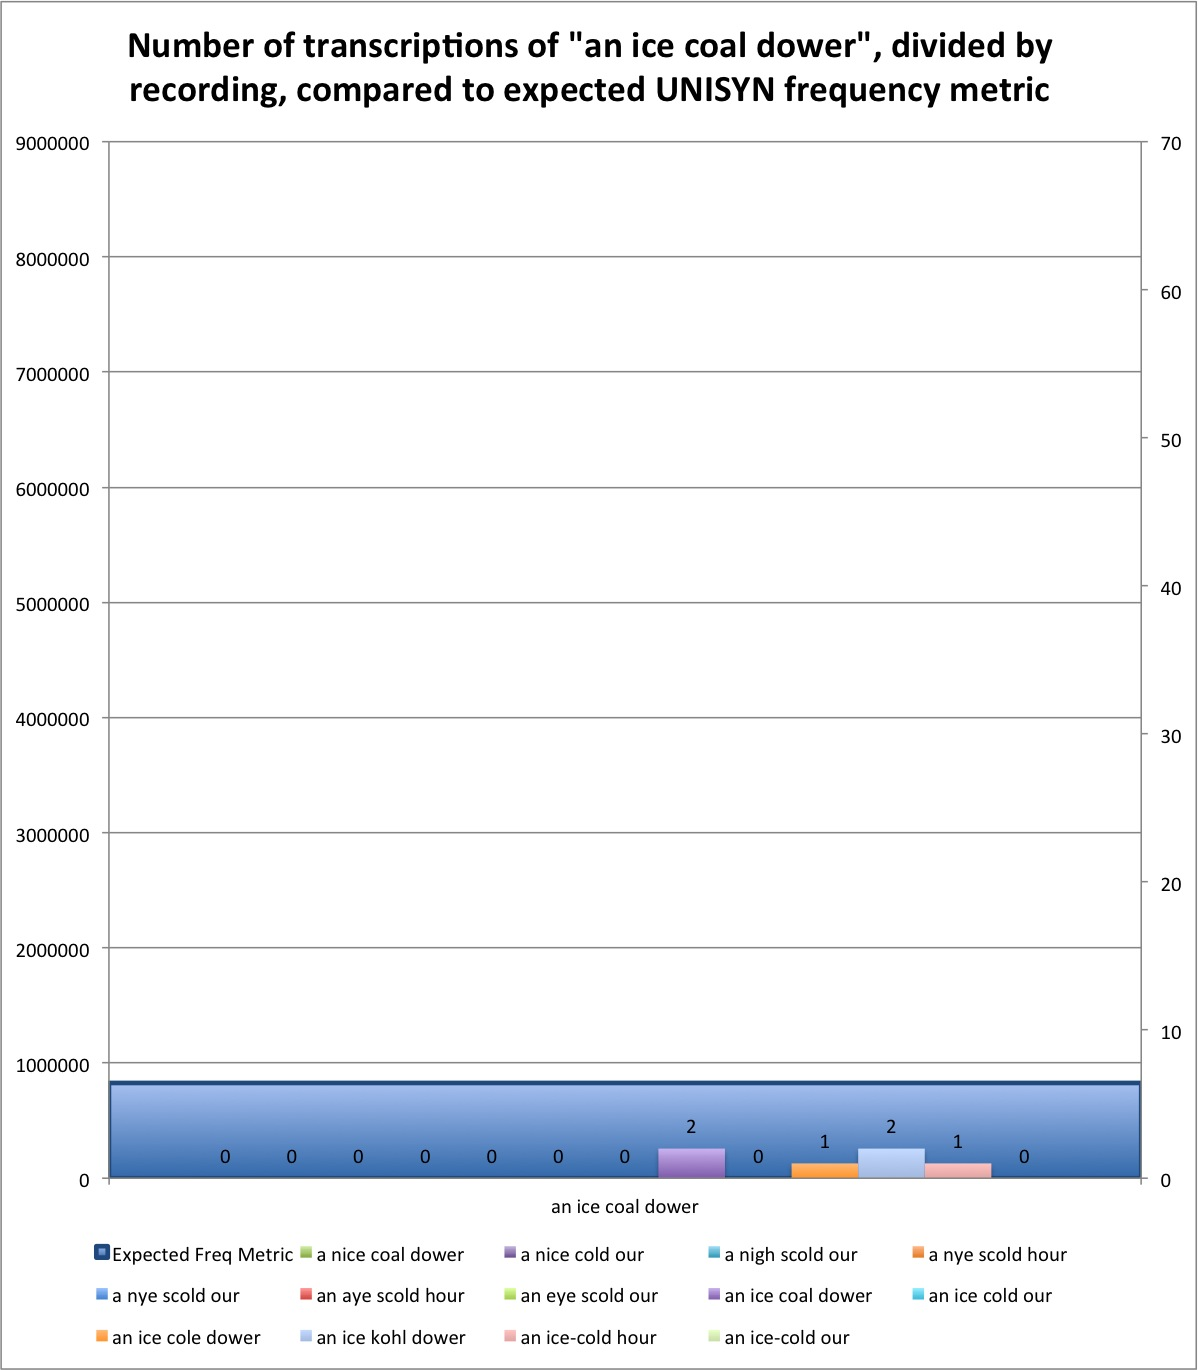
\includegraphics[width=\textwidth]{TranscriptionCountPerRecording_anIceCoalDower.jpg}
\captionfonts
\caption[Transcription Count Per Recording for the transcribed phrase ``an ice coal dower'']{ This graph represents all transcriptions of the phrase ``an ice coal dower'', divided into columns based on what recording were transcribed as ``an ice coal dower''. The large blue bar in the background shows the predicted frequency metric for the phrase in question.}
\label{fig:results:transcriptionCountPerRecordingAnIceCoalDower}
\end{figure}







\subsection{Transcription Breakdown By Country}
\label{results:transcriptionsByCountry}


When comparing transcriptions from countries where English is the dominant language (as shown in figure ~\ref{fig:results:EnglishDominantPieChart}) to those from countries where it is not (as shown in figure ~\ref{fig:results:NonNativePieChart}), we can make some interesting observations.  

\begin{figure}
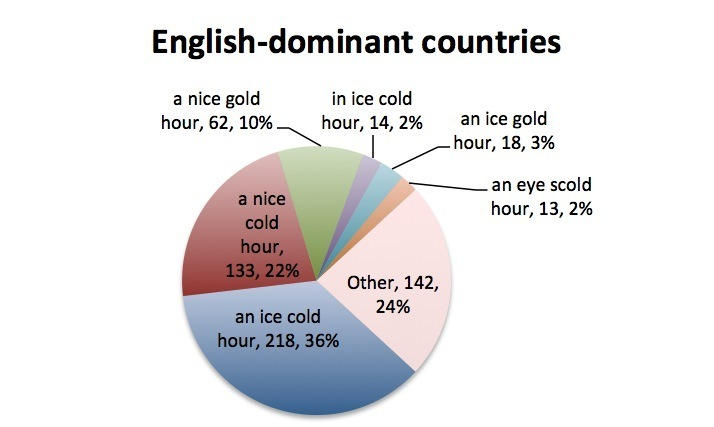
\includegraphics[width=\textwidth]{PieChart-EnglishDominantCountries-nobar.jpg}
\captionfonts
\caption[Pie Chart of transcriptions from countries that are primarily English-speaking]{ Pie Chart of transcriptions from countries that are primarily English-speaking.}
\label{fig:results:EnglishDominantPieChart}
\end{figure}

\begin{figure}
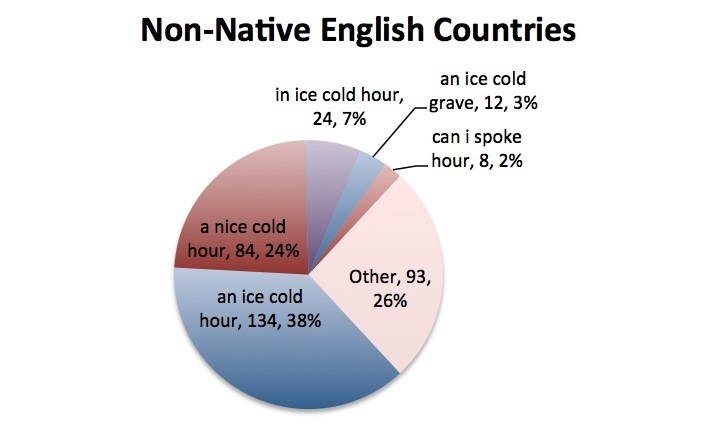
\includegraphics[width=\textwidth]{PieChart-NonNativeEnglishCountries-nobar.jpg}
\captionfonts
\caption[Pie Chart of transcriptions from countries that are Non-native English speakers]{ Pie Chart of transcriptions from countries that are Non-native English speakers.}
\label{fig:results:NonNativePieChart}
\end{figure}

\begin{enumerate}

\item The most common transcription for both is ``an ice cold hour'', with \percentTranscriptionsPerCountryAnIceColdHourEnglishDominant\% native-speaker transcriptions ( \transcriptionsPerCountryAnIceColdHourEnglishDominant) and \percentTranscriptionsPerCountryANiceColdHourNonNative\% non-native ( \transcriptionsPerCountryAnIceColdHourNonNative).

\item The second most common transcription is also the same for both (``a nice cold hour''), but it accounts for a larger percentage of the non-native pie ( \percentTranscriptionsPerCountryANiceColdHourNonNative\% compared to the native \percentTranscriptionsPerCountryANiceColdHourEnglishDominant\% ).

\item The third most common transcription differs for native and non-native speakers. 

Native speakers transcribed ``a nice gold hour'' \transcriptionsPerCountryANiceGoldHourEnglishDominant times, accounting for \percentTranscriptionsPerCountryANiceGoldHourEnglishDominant\% of all native transcriptions. In comparison, only \transcriptionsPerCountryANiceGoldHourNonNative non-native speaker transcribed that phrase, for a measley \percentTranscriptionsPerCountryANiceGoldHourNonNative\% of total non-native transcriptions. 

This brings up an interesting data point---the third most popular transcription for native speakers barely shows up at all for non-native transcribers. There may be something about common phoneme substitution that native speakers pick up on that non-natives do not; specifically, a cold/gold merger.  

 The third most common transcription for non-native speakers is ``in ice cold hour'', which was transcribed \transcriptionsPerCountryInIceColdHourNonNative times, and makes up \percentTranscriptionsPerCountryInIceColdHourNonNative\% of non-native transcriptions.  This phrase was the fifth most common transcription for native speakers, with \transcriptionsPerCountryInIceColdHourEnglishDominant transcriptions making up \percentTranscriptionsPerCountryInIceColdHourEnglishDominant\% of total transcriptions.  

\item The fourth most common transcription for native speakers was ``an ice gold hour'', getting \percentTranscriptionsPerCountryAnIceGoldHourEnglishDominant\% of the total with \transcriptionsPerCountryAnIceGoldHourEnglishDominant transcriptions (by 14 unique transcribers).  This phrase was not transcribed by any non-native speakers. This exhibits the same phone/phoneme substitution that we saw with ``a nice gold hour''.

The fourth most common phrase for non-native speakers, ``an ice cold grave'', was only transcribed by one unique worker, and as such, is not going to be taken into serious consideration. The fifth most common phrase, ``can I spoke hour'', was also only transcribed by one unique worker, and so also cannot be taken into serious consideration.


\end{enumerate}

